%!TEX root = ../project.tex
\part{Design}

%%%
\section{Overall System Design}

\begin{tabular}{|c|c|c|c|}
	\hline
	Inputs & Processes & Storage & Outputs \\ \hline
	Body Parameters & Trajectory Calculations 
		& Current State & Graphical Output \\
	Number of Bodies & Position Calculations 
		& Initial State & Coordinates of Bodies \\ 
	& Graphical Processing && Velocity of Bodies \\\hline
	

	
\end{tabular}

%%%
\section{Human Computer Interface}

\begin{figure}[h!]
	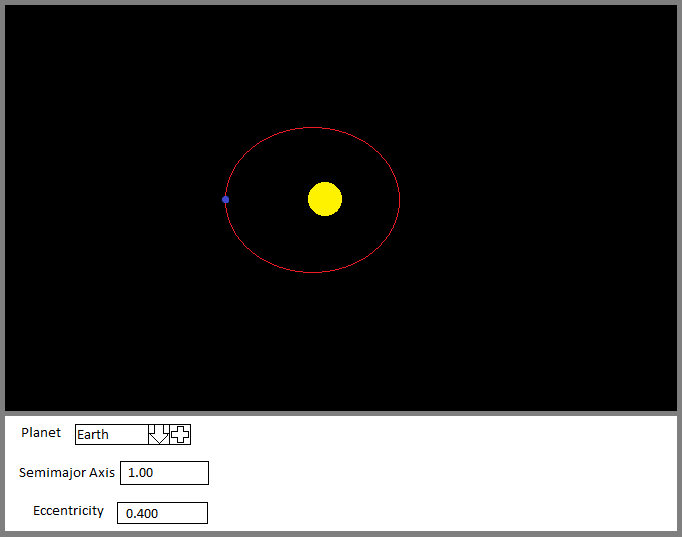
\includegraphics[width=\textwidth]{./img/interface.png}
	\caption{A mockup of the interface}
	\label{fig:hci}
\end{figure}

This is a basic mockup of what I intend for the interface to look like. It looks
quite similar to the old system's interface, so it will be familiar to the user
and they won't have to learn a lot in order to use it.

%%%
\section{Hardware Specification}

My program needs to run on the computers at school, which have:
\begin{description}
	\item[Processor:] Intel Core i3 @ 3.3GHz
	\item[RAM:] 4GB
	\item[Graphics:] Intel HD 2000
	\item[Operating System:] Windows 7
\end{description}

%%%
\section{System Flowchart}

\begin{figure}[h]
	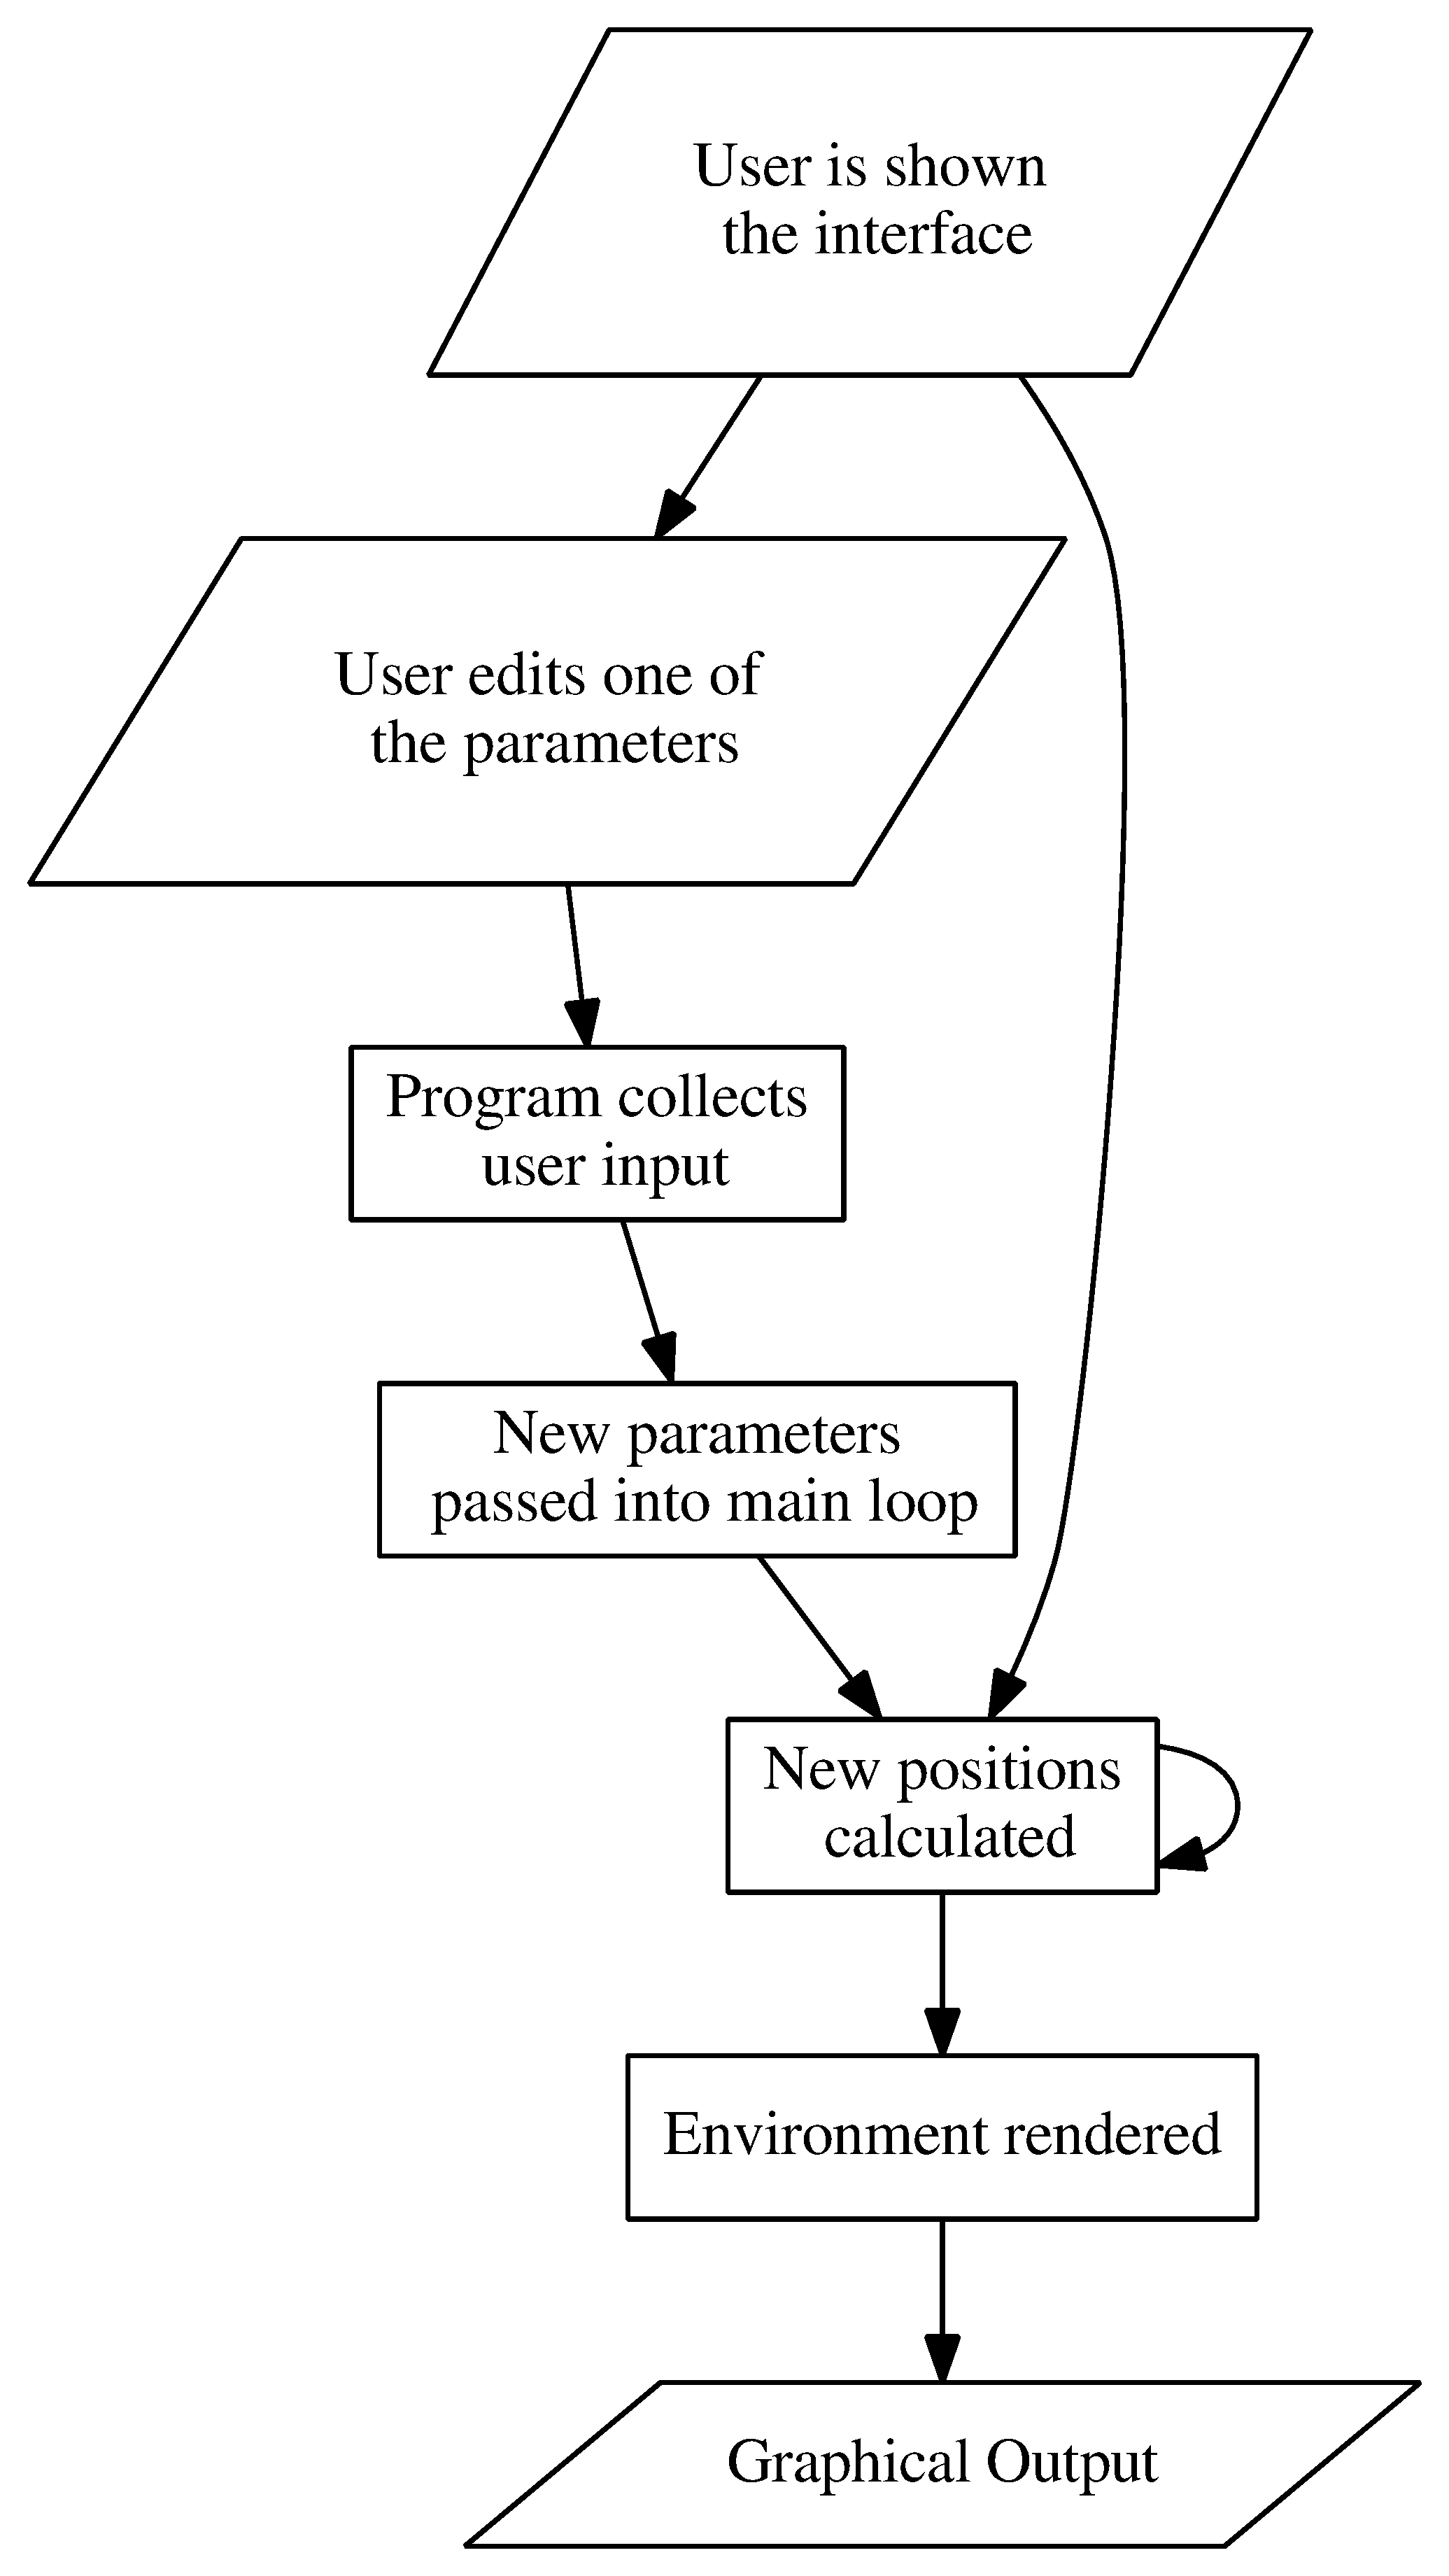
\includegraphics[scale=0.23]{./img/flow.eps}
	\label{fig:flow}	
\end{figure}

%%%
\section{Possible Algorithms to Use}

A big part of my program is the actual simulation of the orbits of some
simulated planets. To simulate and orbit a complex algorithm is required, and
there's a few different ones to choose from.

The Barnes-Hut Tree is a method for performing N-Body simulations, which means
that every body in the simulation will be interacting with every other body.
This, however, isn't very useful for a basic model of a simulation of a solar
system, as the planets generally don't interact with each other very much. It
will allow for more complex simulations, but this isn't necessary for my
project.

The simulation can be simplified to a two body problem, between one planet and
the sun, because the planets aren't affecting each other. This can then be
further simplified to a one body problem, because the sun is much more massive
than a planet, so it can be thought of as the centre of mass. 

Newton's \emph{law of universal gravitation} states that two bodies, with masses
$m_1$ and $m_2$, separated my $r$ are attracted to each other with equal and
opposite forces directed along the line joining the bodies. The magnitude of
this force is given by:

\begin{equation}
	F = G (\frac{m_1 m_2}{r^2})	
\end{equation}

where G is the constant of gravitation (approx. $6.67 N-m^2/kg^2$). We can then
ignore one of the masses, because its significantly less than the other, and
calculate the acceleration towards the object using:

\begin{equation}
	g = \frac{GM}{r^2}
\end{equation}

where $g$ is the acceleration due to gravity and M is the mass of the larger
body. The new position of the body can then be calculated using its current
position and velocity.

\begin{pseudocode}{calc-new-pos}{pos, vel, parentbody}
	r \GETS dist(pos, parentbody)	 \\
	g \GETS (G \cdot parentmass)/r^2 \\
	newvel \GETS vel + g \\
	\RETURN {pos + (newvel \cdot interval)}
\end{pseudocode}
